\chapter{Mengelola Paket Menggunakan npm}

\section{Apakah npm Itu?}

\index{npm}Node.js memungkinkan developer untuk mengembangkan aplikasi secara modular dengan memisahkan berbagai komponen \textit{reusable code} ke dalam pustaka (\textit{library}). Berbagai pustaka tersebut bisa diperoleh di \url{http://npmjs.org}. Node.js menyediakan perintah \textit{npm} untuk mengelola paket pustaka di repositori tersebut. Untuk menggunakan utilitas ini, pemrogram harus terkoneksi dengan Internet.

\section{Menggunakan npm}

Saat melakukan instalasi Node.js, secara otomatis \textit{npm} akan disertakan. Dengan perintah \textit{npm} tersebut, seorang pemrogram bisa mengelola pustaka yang tersedia di repositori. Jika pemrogram mempunya pustakan yang bisa digunakan oleh orang lain, maka pemrogram yang bersangkutan juga bisa menyimpan pustaka tersebut ke dalam repositori sehingga memungkinkan untuk diinstall oleh pemrogram-pemrogram lain di seluruh dunia. Sintaksis lengkap dari penggunaan perintah \textit{npm} ini adalah sebagai berikut\footnote{beberapa bagian tertulis spesifik lokasi direktori di komputer yang digunakan penulis}:

\lstset{language=bash,caption=Sintaksis lengkap perintah \textit{npm}}
\begin{lstlisting}
$ npm --help

Usage: npm <command>

where <command> is one of:
    add-user, adduser, apihelp, author, bin, bugs, c, cache,
    completion, config, ddp, dedupe, deprecate, docs, edit,
    explore, faq, find, find-dupes, get, help, help-search,
    home, i, info, init, install, isntall, la, link, list, ll,
    ln, login, ls, outdated, owner, pack, prefix, prune,
    publish, r, rb, rebuild, remove, restart, rm, root,
    run-script, s, se, search, set, show, shrinkwrap, star,
    start, stop, submodule, tag, test, tst, un, uninstall,
    unlink, unpublish, unstar, up, update, version, view,
    whoami

npm <cmd> -h     quick help on <cmd>
npm -l           display full usage info
npm faq          commonly asked questions
npm help <term>  search for help on <term>
npm help npm     involved overview

Specify configs in the ini-formatted file:
    /home/bpdp/.npmrc
or on the command line via: npm <command> --key value
Config info can be viewed via: npm help config

npm@1.1.70 /home/bpdp/software/node-v0.8.16-linux-x86/lib/node_modules/npm
\end{lstlisting}

Pada bagian berikut, kita akan membahas lebih lanjut penggunaan perintah \textit{npm} tersebut.

\subsection{Instalasi Paket}

\index{npm!install paket}npm sebenarnya bukan merupakan singkatan dari \textit{Node Package Manager}, meskipun seringkali orang menterjemahkan dengan singkatan tersebut dan npm seharusnya ditulis dalam huruf kecil semua seperti yang dijelaskan pada FAQ (\textit{Frequently Asked Questions})\footnote{\url{https://npmjs.org/doc/faq.html}}. npm merupakan bilah alat berbasis baris perintah, dijalankan melalui shell atau \textit{command prompt}. Sama seperti kebanyakan bilah alat berbasis baris perintah lain, npm memiliki struktur perintah \textit{npm perintah argumen}. Installasi paket pustaka dilakukan dengan perintah berikut :

\lstset{language=bash,caption=Cara install paket menggunakan npm}
\begin{lstlisting}
$ npm install foo
\end{lstlisting}

Perintah diatas akan memasang versi terakhir dari paket pustaka foo. Selain itu \textit{npm} juga dapat memasang paket pustaka langsung pada sebuah folder, tarball atau tautan untuk sebuah tarball.

\subsection{Struktur Instalasi Paket Node.js}

\index{npm!Struktur paket}Dalam installasi paket pustaka, berkas-berkas akan terletak dalam folder lokal aplikasi \textit{node\_modules}. Pada mode installasi paket pustaka global (dengan -g atau --global dibelakang baris perintah), paket pustaka akan dipasang pada \textit{/usr/lib/node\_modules} (dengan lokasi installasi Node.js standar). Mode global memungkinkan paket pustaka digunakan tanpa memasang paket pustaka pada setiap folder lokal aplikasi. Mode global ini juga membutuhkan hak administrasi lebih (sudo atau root) dari pengguna agar dapat menulis pada lokasi standar. 

Jika berada pada direktori \$HOME, maka paket-paket npm tersebut akan terinstall di \$HOME/.npm, sedangkan jika kita berada di luar direktori \$HOME, maka paket-paket tersebut akan terinstall di \$CWD/node\_modules (\$CWD = \textit{Current Working Directory} - direktori aktif saat ini). Daftar paket pustaka yang terpasang dapat dilihat menggunakan perintah berikut:

\lstset{language=bash,caption=Argumen npm untuk melihat daftar paket terpasang}
\begin{lstlisting}
$ npm ls
\end{lstlisting}

Selain melihat daftar paket pustaka yang digunakan dalam aplikasi maupun global, perintah diatas juga akan menampilkan paket dependensi dalam struktur pohon. Gambar~\ref{fig:npmls} berikut menampilkan contoh struktur instalasi dari aplikasi yang sudah kita buat menggunakan ExpressJS (lihat bab 1):

  \begin{figure}
    \begin{center}
      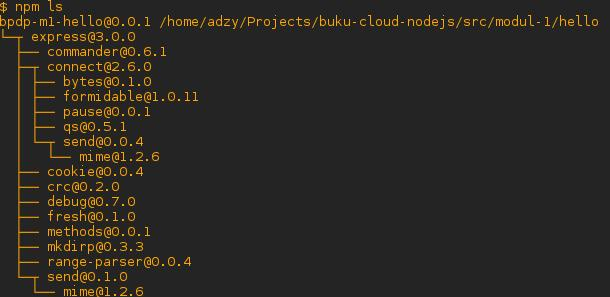
\includegraphics[scale=0.5]{images/npmls.jpg}
    \end{center}
    \caption{Hasil perintah npm ls}
    \label{fig:npmls}
  \end{figure}

\subsection{Menghapus Paket / \textit{Uninstall}}

\index{npm!Hapus paket}Menghapus paket pustaka menggunakan npm pada dasarnya hampir sama dengan saat memasang paket, namun dengan perintah \textit{uninstall}. Berikut perintah lengkapnya.

\lstset{language=bash,caption=Perintah menghapus paket di npm}
\begin{lstlisting}
$ npm uninstall foo
\end{lstlisting}

Paket pustaka foo dalam lokal aplikasi akan dihapus, jika menggunakan hak administrasi sudo atau root maka akan menghapus dari installasi global.

\subsection{Mencari Paket}

\index{npm!Cari paket}Untuk mencari paket, gunakan argumen \textit{search} dan nama atau bagian dari nama paket yang dicari. Contoh berikut ini akan mencari paket dengan kata kunci 'sha512' (tampilan berikut merupakan tampilan yang terpotong):

\lstset{language=bash,caption=Perintah menghapus paket di npm}
\begin{lstlisting}
$ npm search sha512
npm http GET https://registry.npmjs.org/-/all/since?stale=...
npm http 200 https://registry.npmjs.org/-/all/since?stale=...
NAME    DESCRIPTION                                       ...
krypto  High-level crypto library, making the core crypto ...
pwhash  Generate password hashes from the command line.   ...
\end{lstlisting}

Setelah menemukan paketnya, pemrogram bisa menginstall langsung ataupun melihat informasi lebih lanjut tentang pustakan tersebut.

\subsection{Menampilkan Informasi Paket}

\index{npm!Info paket}Setelah mengetahui nama paket, pemrogram bisa memperoleh informasi lebih lanjut dalam format JSON menggunakan parameter \textit{view}. Contoh dibawah ini menampilkan rincian dalam format JSON dari paket \textit{arango.client}:

\lstset{language=bash,caption=Menampilkan rincian suatu paket dalam format JSON}
\begin{lstlisting}
$ npm view arango.client
npm http GET https://registry.npmjs.org/arango.client
npm http 304 https://registry.npmjs.org/arango.client

{ name: 'arango.client',
  description: 'ArangoDB javascript client',
  'dist-tags': { latest: '0.5.6' },
  versions: 
   [ '0.3.1',
     '0.3.2',
     '0.4.0',
     '0.5.0',
     '0.5.1',
     '0.5.4',
     '0.5.6' ],
  maintainers: 'kaerus <anders@kaerus.com>',
  time: 
   { '0.3.1': '2012-08-09T12:04:34.594Z',
     '0.3.2': '2012-08-09T12:49:02.322Z',
     '0.4.0': '2012-09-17T10:44:43.187Z',
     '0.5.0': '2012-10-01T14:51:32.668Z',
     '0.5.1': '2012-10-03T22:11:58.376Z',
     '0.5.4': '2012-10-16T09:45:37.477Z',
     '0.5.6': '2012-10-26T17:34:28.491Z' },
  author: 'Kaerus <contact@kaerus.com> (http://kaerus.com)',
  repository: 
   { type: 'git',
     url: 'git://github.com/kaerus/arango-client.git' },
  version: '0.5.6',
  keywords: 
   [ 'arangodb',
     'nosql',
     'qunit',
     'amd' ],
  contributors: 'anders elo <anders@kaerus.com>',
  dependencies: { amdefine: '>=0.0.2' },
  devDependencies: { requirejs: '>=2.0.6' },
  bugs: { url: 'https://github.com/kaerus/arango-client/issues' },
  main: 'index.js',
  license: 'MIT',
  dist: 
   { shasum: '48279e7cf9ea0b4b6766f09671224c46d6e716b0',
     tarball: 'http://registry.npmjs.org/arango.client/-/arango.client-0.5.6.tgz' },
  directories: {} }
\end{lstlisting}

\subsection{Memperbaharui Paket}

\index{npm!Update paket}Jika terdapat versi baru, kita bisa memperbaharui secara otomatis menggunakan argumen \textit{update} berikut ini:

\lstset{language=bash,caption=Memperbaharui paket lokal}
\begin{lstlisting}
npm update
\end{lstlisting}

\lstset{language=bash, caption=Memperbaharui paket secara global}
\begin{lstlisting}
npm update -g
\end{lstlisting}
